\section{Mappa}

Viene discussa ora la realizzazione della mappa di una regione di cielo, in corrispondenza del cigno. L'attenzione è posta nell'intervallo di valori tra 38 e 47 deg di declinazione (Dec), e 290 e 320 deg di ascensione retta (RA).
\\\\
Per ottenere i dati di interesse, ad ogni puntamento della parabole si sceglie di lasciare fisso il valore di declinazione lasciando variare l'ascensione retta. Di conseguenza ciascuna osservazione fornirà una riga orizzontale della mappa. Ripetendo i campionamenti su vari giorni è possibile costruire la mappa completa. 
\\\\
Le coordinate, in azimuth ed elevazione, da fornire alla parabola vengono ricavate utilizzando lo stesso programma descritto in \ref{Programma coordinate}; scegliendo il valore di declinazione giornalmente, ponendo l' RA a 308 $^{\circ}$, valore di coordinata celeste del cigno. Osservazioni della durata di 3:00 h permetto di spaziare sul range di 30 $^{\circ}$ di RA citato precedentemente.



\subsection{Composizione della mappa}

Per ogni osservazione vengono in totale utilizzati 32 file, le rispettive coordinate azimuth ed elevazione sono sempre ricavabili sfruttando la funzione $transform\_to$. Per ogni file viene eseguita l'analisi delle velocità descritta nella sezione \ref{Analisi Dati e Velocità}. D'interesse è il valore della temperatura di brillanza in corrispondenza del primo picco osservato. 
\\\\
Analizzando ognuno dei set di dati, si possono comporre le varie righe, corrispondenti a declinazioni diverse, attraverso la funzione di stampa $\textit{imshow}$, presenta nella libreria $\textit{mathplotlib}$ di python. Nel dettaglio, è possibile passare, come argomento della funzione, la variabile $\textit{extent}$, ovvero le coordinate che compongono la griglia, nel nostro caso [290-320; 38-47].
\\\\
Il risultato finale è qui riportato: 

\begin{figure}[H]
	\centering
	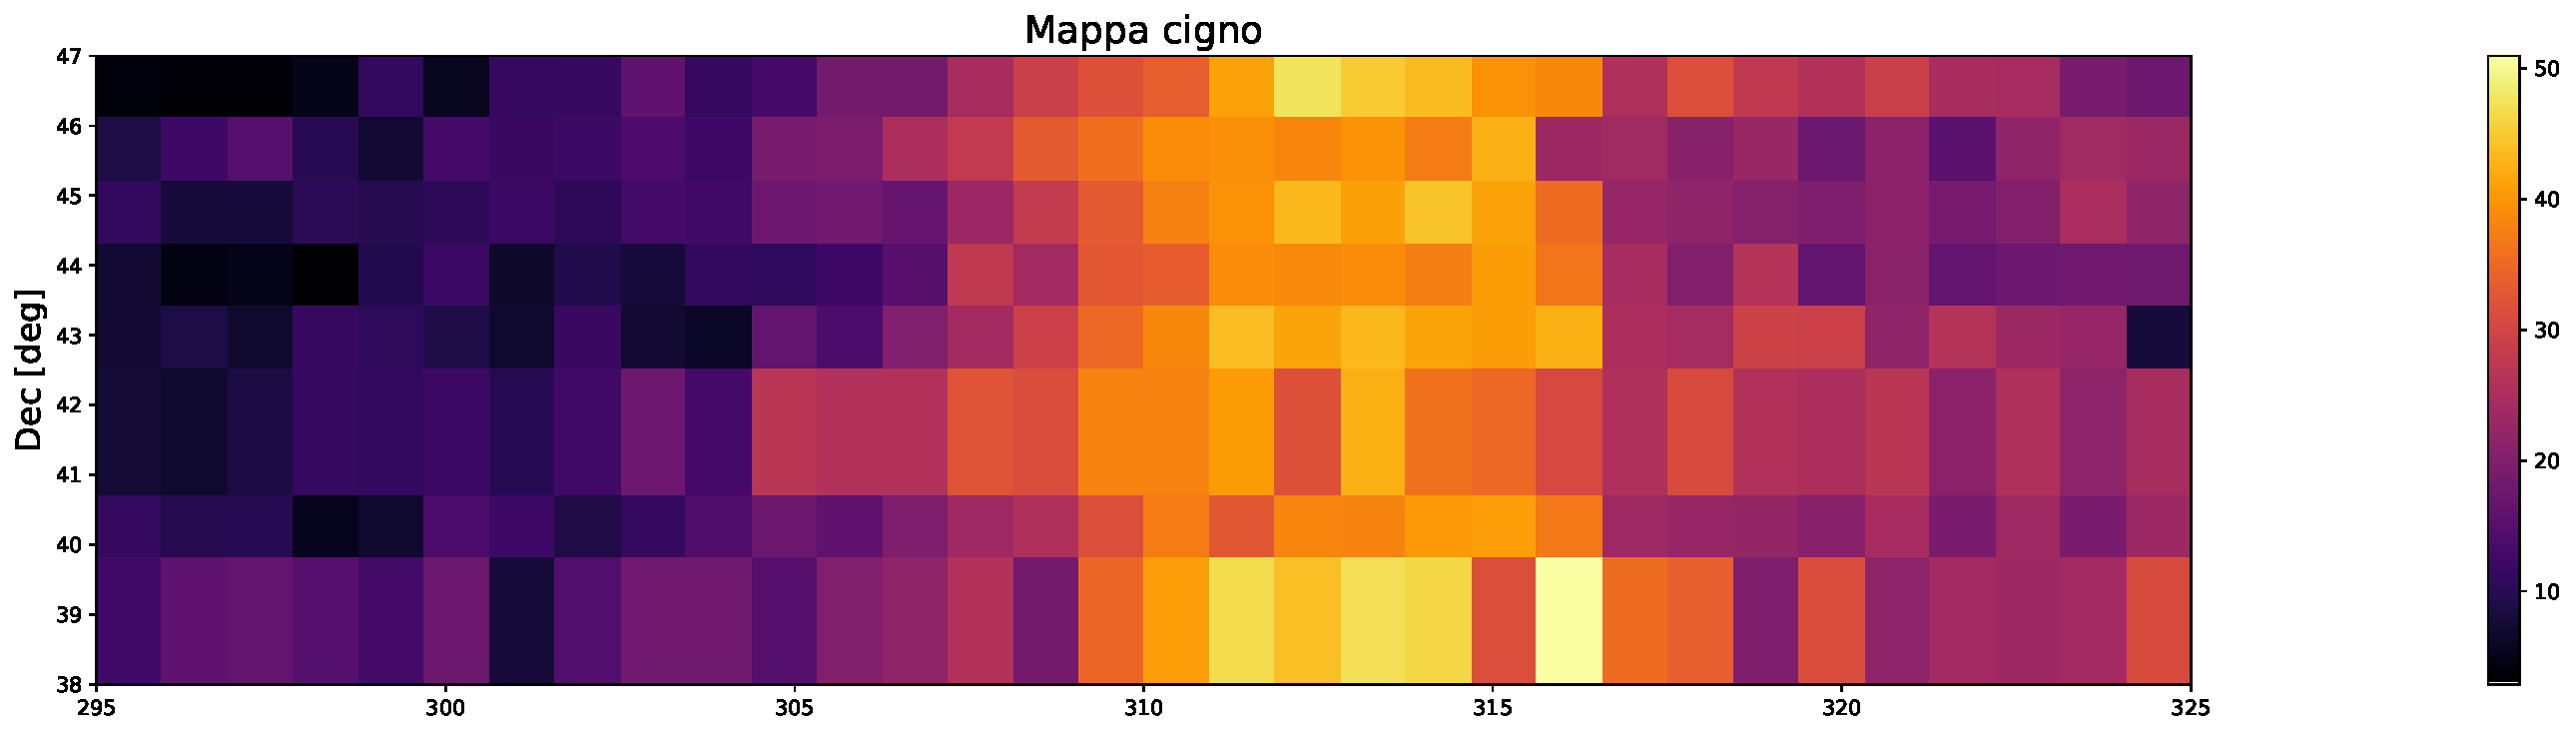
\includegraphics[scale=0.4]{Mappa_grezza.pdf}
	\caption{Mappa del cigno, le intensità dei colori corrispondo ai valori della temperatura di brillanza come indicato nella barra a lato espressa in Kelvin}
    	\label{fig:Mappa_grezza}
\end{figure}

\subsection{Processo di smoothing della mappa}

Il risultato ottenuto, mostrato in figura \ref{fig:Mappa_grezza}, è notevolmente grezzo e irregolare. Per tale motivazione, viene attuata una procedura di smoothing della mappa, al fine di ottenere un risultato continuo ed uniforme.
\\\\
La procedura si dipana in due passaggi. Il primo step consiste nell'applicare una convoluzione tra il set di dati e un kernel gaussiano bidimensionale. Ci si avvale direttamente della funzione $\textit{convolve}$ ottenendo la seguente mappa:

\begin{figure}[H]
	\centering
	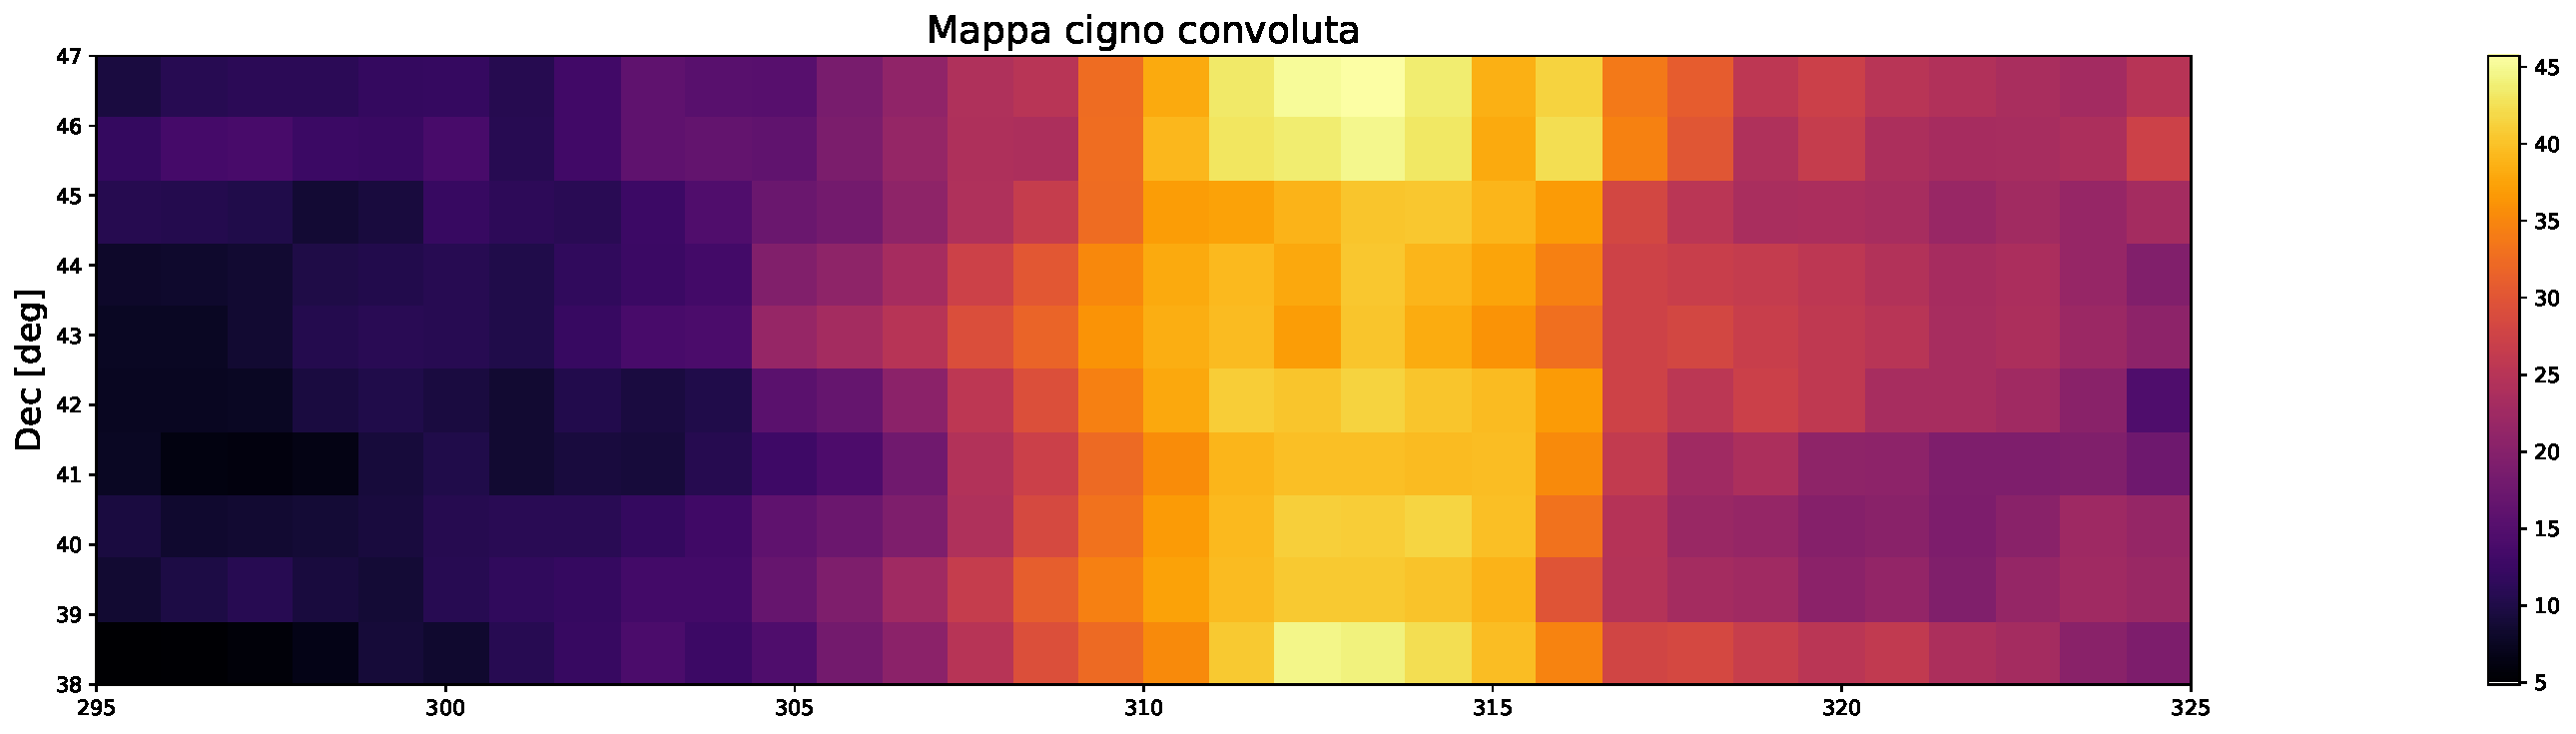
\includegraphics[scale=0.4]{Mappa_convolve.pdf}
	\caption{Mappa del cigno convoluta con un kernel gaussiano}
    	\label{fig:Mappa_convolve}
\end{figure}

Si può notare un minor distacco tra i colori, i.e. temperatura, associati ai diversi pixel.
\\\\
Il secondo step ha il fine di rimuovere il distacco dato dalla griglia dei pixel passando a un andamento maggiormente omogeneo. La già utilizzata funzione $\textit{imshow}$ permette di eseguire un'interpolazione tra un pixel e i suoi adiacenti. Viene qui riportato la mappa finale, ottenibile interpolando le funzioni di Bessel; 

\begin{figure}[H]
	\centering
	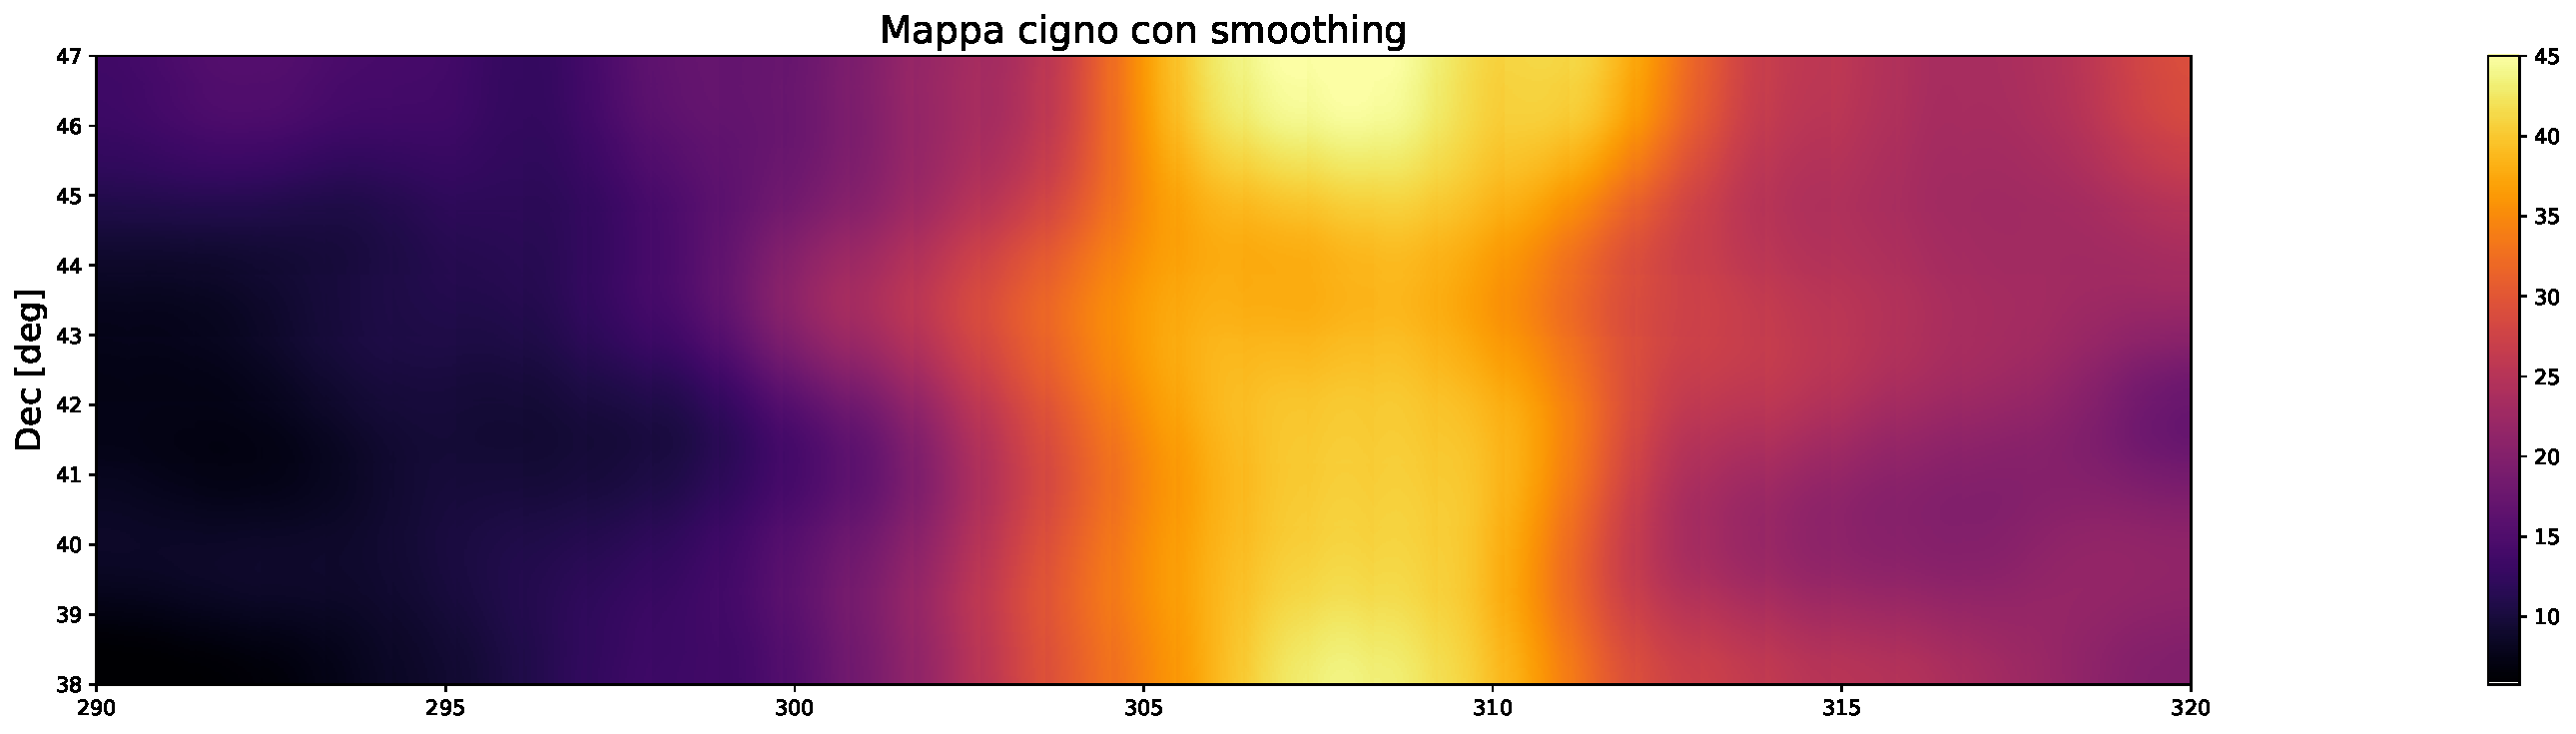
\includegraphics[scale=0.4]{Mappa_finale.pdf}
	\caption{Mappa del cigno a cui è stato applicato il processo di smoothing}
    	\label{fig:Mappa_finale}
\end{figure}

Si noti la corrispondenza tra i punti in cui sono presenti i valori maggiori di temperatura di brillanza e le coordinate galattiche della regione del cigno, fulcro dello studio eseguito.


